\documentclass{standalone}
\usepackage{tikz}
\usetikzlibrary{patterns, positioning}
\usepackage[sfdefault]{ClearSans} %% option 'sfdefault' activates Clear Sans as the default text font
\usepackage[T1]{fontenc}

\begin{document}
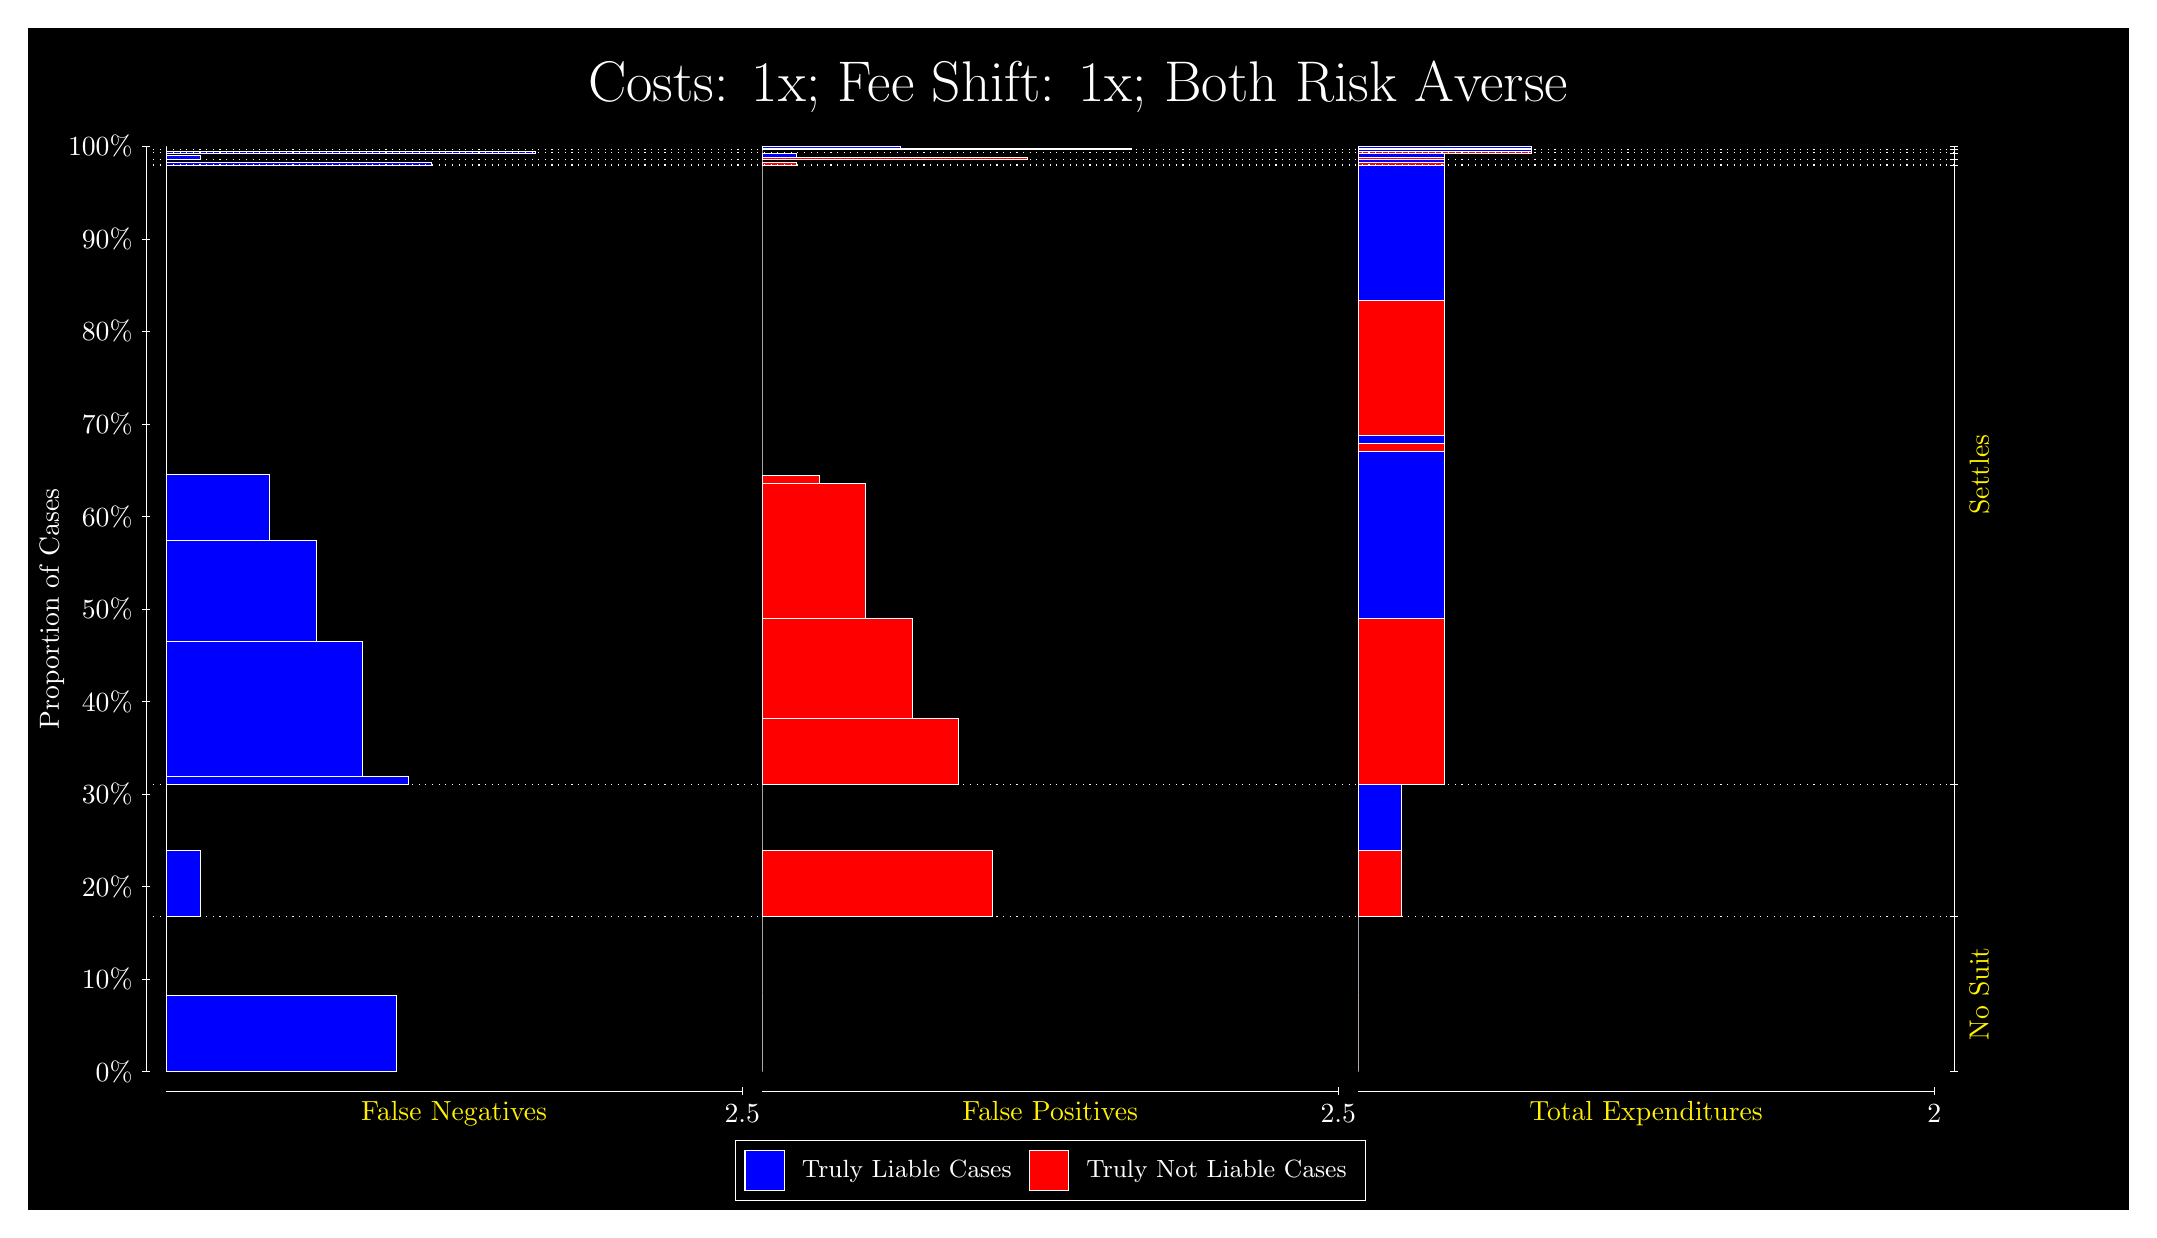
\begin{tikzpicture}
\draw[fill=black] (0,0) rectangle (26.667,15);
\draw[text=white] (0,13.5) rectangle (26.667,15) node[midway] {\huge Costs: 1x; Fee Shift: 1x; Both Risk Averse};
\draw[white, very thin] (1.5,1.75) -- (1.5,13.5);
\node[rotate=90, text=white, anchor=center] at (0.3, 7.625) {Proportion of Cases};
\draw[white, very thin] (1.45,1.75) -- (1.55,1.75);
\node[text=white, anchor=east] at (1.45, 1.75) {0\%};
\draw[white, very thin] (1.45,2.925) -- (1.55,2.925);
\node[text=white, anchor=east] at (1.45, 2.925) {10\%};
\draw[white, very thin] (1.45,4.1) -- (1.55,4.1);
\node[text=white, anchor=east] at (1.45, 4.1) {20\%};
\draw[white, very thin] (1.45,5.275) -- (1.55,5.275);
\node[text=white, anchor=east] at (1.45, 5.275) {30\%};
\draw[white, very thin] (1.45,6.45) -- (1.55,6.45);
\node[text=white, anchor=east] at (1.45, 6.45) {40\%};
\draw[white, very thin] (1.45,7.625) -- (1.55,7.625);
\node[text=white, anchor=east] at (1.45, 7.625) {50\%};
\draw[white, very thin] (1.45,8.8) -- (1.55,8.8);
\node[text=white, anchor=east] at (1.45, 8.8) {60\%};
\draw[white, very thin] (1.45,9.975) -- (1.55,9.975);
\node[text=white, anchor=east] at (1.45, 9.975) {70\%};
\draw[white, very thin] (1.45,11.15) -- (1.55,11.15);
\node[text=white, anchor=east] at (1.45, 11.15) {80\%};
\draw[white, very thin] (1.45,12.325) -- (1.55,12.325);
\node[text=white, anchor=east] at (1.45, 12.325) {90\%};
\draw[white, very thin] (1.45,13.5) -- (1.55,13.5);
\node[text=white, anchor=east] at (1.45, 13.5) {100\%};

\draw[white, very thin] (24.457,1.75) -- (24.457,13.5);
\draw[white, very thin] (24.407,1.75) -- (24.507,1.75);
\node[anchor=west] at (24.407, 1.75) {};
\draw[white, very thin] (24.407,3.721) -- (24.507,3.721);
\node[anchor=west] at (24.407, 3.721) {};
\draw[white, very thin] (24.407,5.3996) -- (24.507,5.3996);
\node[anchor=west] at (24.407, 5.3996) {};
\draw[white, very thin] (24.407,13.263) -- (24.507,13.263);
\node[anchor=west] at (24.407, 13.263) {};
\draw[white, very thin] (24.407,13.332) -- (24.507,13.332);
\node[anchor=west] at (24.407, 13.332) {};
\draw[white, very thin] (24.407,13.416) -- (24.507,13.416);
\node[anchor=west] at (24.407, 13.416) {};
\draw[white, very thin] (24.407,13.458) -- (24.507,13.458);
\node[anchor=west] at (24.407, 13.458) {};
\draw[white, very thin] (24.407,13.5) -- (24.507,13.5);
\node[anchor=west] at (24.407, 13.5) {};

\draw[white, very thin, fill=blue] (1.75,1.75) rectangle (4.6775,2.7205);
\draw[white, very thin, fill=red] (1.75,2.7205) rectangle (1.75,3.721);
\draw[white, very thin, fill=blue] (1.75,3.721) rectangle (2.1891,4.5603);
\draw[white, very thin, fill=red] (1.75,4.5603) rectangle (1.75,5.3996);
\draw[white, very thin, fill=blue] (1.75,5.3996) rectangle (4.8239,5.4934);
\draw[white, very thin, fill=blue] (1.75,5.4934) rectangle (4.2384,7.2171);
\draw[white, very thin, fill=blue] (1.75,7.2171) rectangle (3.6529,8.4954);
\draw[white, very thin, fill=blue] (1.75,8.4954) rectangle (3.0674,9.3347);
\draw[white, very thin, fill=red] (1.75,9.3347) rectangle (1.75,13.263);
\draw[white, very thin, fill=blue] (1.75,13.263) rectangle (5.1167,13.297);
\draw[white, very thin, fill=red] (1.75,13.297) rectangle (1.75,13.332);
\draw[white, very thin, fill=blue] (1.75,13.332) rectangle (2.1891,13.382);
\draw[white, very thin, fill=red] (1.75,13.382) rectangle (1.75,13.416);
\draw[white, very thin, fill=blue] (1.75,13.416) rectangle (6.4341,13.436);
\draw[white, very thin, fill=red] (1.75,13.436) rectangle (1.75,13.458);
\draw[white, very thin, fill=red] (1.75,13.458) rectangle (1.75,13.476);
\draw[white, very thin, fill=blue] (1.75,13.476) rectangle (1.75,13.5);
\draw[white, very thin, fill=red] (9.3189,1.75) rectangle (9.3189,2.7506);
\draw[white, very thin, fill=blue] (9.3189,2.7506) rectangle (9.3189,3.721);
\draw[white, very thin, fill=red] (9.3189,3.721) rectangle (12.246,4.5603);
\draw[white, very thin, fill=blue] (9.3189,4.5603) rectangle (9.3189,5.3996);
\draw[white, very thin, fill=red] (9.3189,5.3996) rectangle (11.807,6.2389);
\draw[white, very thin, fill=red] (9.3189,6.2389) rectangle (11.222,7.5115);
\draw[white, very thin, fill=red] (9.3189,7.5115) rectangle (10.636,9.2259);
\draw[white, very thin, fill=red] (9.3189,9.2259) rectangle (10.051,9.3275);
\draw[white, very thin, fill=blue] (9.3189,9.3275) rectangle (9.3189,13.263);
\draw[white, very thin, fill=red] (9.3189,13.263) rectangle (9.758,13.297);
\draw[white, very thin, fill=blue] (9.3189,13.297) rectangle (9.3189,13.332);
\draw[white, very thin, fill=red] (9.3189,13.332) rectangle (12.686,13.365);
\draw[white, very thin, fill=blue] (9.3189,13.365) rectangle (9.758,13.416);
\draw[white, very thin, fill=red] (9.3189,13.416) rectangle (9.3189,13.437);
\draw[white, very thin, fill=blue] (9.3189,13.437) rectangle (9.3189,13.458);
\draw[white, very thin, fill=red] (9.3189,13.458) rectangle (14.003,13.476);
\draw[white, very thin, fill=blue] (9.3189,13.476) rectangle (11.075,13.5);
\draw[white, very thin, fill=red] (16.888,1.75) rectangle (16.888,2.7506);
\draw[white, very thin, fill=blue] (16.888,2.7506) rectangle (16.888,3.721);
\draw[white, very thin, fill=red] (16.888,3.721) rectangle (17.437,4.5603);
\draw[white, very thin, fill=blue] (16.888,4.5603) rectangle (17.437,5.3996);
\draw[white, very thin, fill=red] (16.888,5.3996) rectangle (17.986,7.5115);
\draw[white, very thin, fill=blue] (16.888,7.5115) rectangle (17.986,9.6291);
\draw[white, very thin, fill=red] (16.888,9.6291) rectangle (17.986,9.7307);
\draw[white, very thin, fill=blue] (16.888,9.7307) rectangle (17.986,9.8245);
\draw[white, very thin, fill=red] (16.888,9.8245) rectangle (17.986,11.539);
\draw[white, very thin, fill=blue] (16.888,11.539) rectangle (17.986,13.263);
\draw[white, very thin, fill=red] (16.888,13.263) rectangle (17.986,13.297);
\draw[white, very thin, fill=blue] (16.888,13.297) rectangle (17.986,13.332);
\draw[white, very thin, fill=red] (16.888,13.332) rectangle (17.986,13.365);
\draw[white, very thin, fill=blue] (16.888,13.365) rectangle (17.986,13.416);
\draw[white, very thin, fill=red] (16.888,13.416) rectangle (19.083,13.437);
\draw[white, very thin, fill=blue] (16.888,13.437) rectangle (19.083,13.458);
\draw[white, very thin, fill=red] (16.888,13.458) rectangle (19.083,13.476);
\draw[white, very thin, fill=blue] (16.888,13.476) rectangle (19.083,13.5);
\draw[white, dotted] (1.5,3.721) -- (24.457,3.721);
\draw[white, dotted] (1.5,5.3996) -- (24.457,5.3996);
\draw[white, dotted] (1.5,13.263) -- (24.457,13.263);
\draw[white, dotted] (1.5,13.332) -- (24.457,13.332);
\draw[white, dotted] (1.5,13.416) -- (24.457,13.416);
\draw[white, dotted] (1.5,13.458) -- (24.457,13.458);
\draw[white, very thin] (1.75,1.5) -- (9.0689,1.5);
\node[text=yellow, anchor=north] at (5.4094, 1.5) {False Negatives};
\draw[white, very thin] (9.0689,1.45) -- (9.0689,1.55);
\node[text=white, anchor=north] at (9.0689, 1.45) {2.5};

\draw[white, very thin] (9.3189,1.5) -- (16.638,1.5);
\node[text=yellow, anchor=north] at (12.978, 1.5) {False Positives};
\draw[white, very thin] (16.638,1.45) -- (16.638,1.55);
\node[text=white, anchor=north] at (16.638, 1.45) {2.5};

\draw[white, very thin] (16.888,1.5) -- (24.207,1.5);
\node[text=yellow, anchor=north] at (20.547, 1.5) {Total Expenditures};
\draw[white, very thin] (24.207,1.45) -- (24.207,1.55);
\node[text=white, anchor=north] at (24.207, 1.45) {2};

\node[text=yellow, centered, rotate=90] at (24.777, 2.7355) {No Suit};

\node[text=yellow, centered, rotate=90] at (24.777, 9.3311) {Settles};





\draw (12.978300999999998,1.5) node[draw=none] (baseCoordinate) {};
\begin{scope}[align=center]
        \matrix[scale=0.5, draw=white, below=0.5cm of baseCoordinate, nodes={draw}, column sep=0.1cm]{
            \node[rectangle, draw, minimum width=0.5cm, minimum height=0.5cm, fill=blue] {}; &
            \node[draw=none, font=\small, text=white] (B) {Truly Liable Cases}; &
            \node[rectangle, draw, minimum width=0.5cm, minimum height=0.5cm, fill=red] {}; &
            \node[draw=none, font=\small, text=white] (B) {Truly Not Liable Cases}; \\
            };
\end{scope}

\end{tikzpicture}
\end{document}